\documentclass[conference]{IEEEtran}
\IEEEoverridecommandlockouts
% The preceding line is only needed to identify funding in the first footnote. If that is unneeded, please comment it out.
\usepackage{cite}
\usepackage{amsmath,amssymb,amsfonts}
\usepackage{algorithmic}
\usepackage{graphicx}
\usepackage{textcomp}
\usepackage{xcolor}
\def\BibTeX{{\rm B\kern-.05em{\sc i\kern-.025em b}\kern-.08em
    T\kern-.1667em\lower.7ex\hbox{E}\kern-.125emX}}
\begin{document}

\title{Sentiment Analysis with Sarcasm Detection\\
}

\author{\IEEEauthorblockN{Ryan Gross}
rgross4@gwmail.gwu.edu
\and
\IEEEauthorblockN{Sam Odle}
samodle@gwmail.gwu.edu
}

\maketitle

\begin{abstract}
The Sentiment Analysis with Sarcasm Detection project aims to outperform current state-of-the-art sentiment analysis systems by fixing a major shortcoming of current algorithms. \\
Current sentiment systems fail to recognize sarcasm, often rendering sentiment scores that are not only inaccurate, but can be the opposite of the author’s actual intended sentiment. This shortcoming is readily apparent when companies use sentiment scores to automatically reply to comments, reviews, and tweets using chatbots. \\
In this experiment, we have combined several techniques for detecting sarcasm and averaged their analysis scores to better inform the final sentiment of the input text. While sentiment accuracy is a purely subjective metric, we will demonstrate results on passages that clearly demonstrate improvements over Google Cloud Platform’s (GCP) Natural Language sentiment analysis results for the same input text. \\
This paper will outline the methodology for each sarcasm detection technique, talk to the strengths and weaknesses of each, and show testing results. Furthermore, it will convince the reader that prioritizing sarcasm detection is essential for sentiment analysis accuracy, especially in real world applications. 

\end{abstract}

\section{Introduction}

This paper’s primary purpose is to convince the reader through examples that today’s Sentiment Analysis systems produce flawed results when sarcasm is present because they do not take it into account when scoring input text. This paper will discuss why that presents problems to businesses of all sizes, again using real world examples. Additionally, the reader will see several potential methods to close this existing gap and will see results that will prove the additional detection of sarcasm improves Sentiment Analysis accuracy. \\
Today, Sentiment Analysis is used by companies all over the world to better understand and connect with their customers. For example, companies will run Sentiment Analysis services against Yelp reviews, Amazon reviews, tweets on Twitter that mention their product or company, and many more sources for customer feedback. Companies also use real-time sentiment analysis services like Contact Lens for Amazon Connect to better serve customers their staff is actively engaged with.\\
With the constant growth of online services, Sentiment Analysis has become an essential tool for customer service organizations.  There simply is too much data for employees to manually review, so Sentiment Analysis services automate the task of bucketing negative and positive reviews. A quick response is important because these reviews are public and will immediately impact other potential customers.  It is also a learning opportunity for the company on how to improve their product or better serve the customer. It may help them identify trends or potential issues that they themselves are unaware of. Identifying a poor review is also an opportunity for a customer representative to assist the customer or provide a refund, which can sometimes lead to the customer improving their review of the product.\\

\begin{figure}[htbp]
\centerline{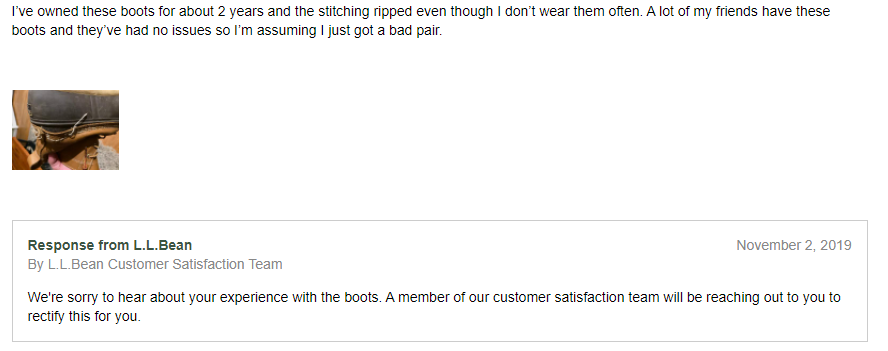
\includegraphics[width=9cm]{image1.png}}
\caption{L.L. Bean Responds to Negative Review}
\label{fig}
\end{figure}

Notice how in Figure 1, above, a customer representative was able to reach out to the customer to apologize and rectify the situation. Understanding customer sentiment also gives companies an opportunity to engage with customers and thank them for their patronage. In the Yelp review (Figure 2), you can see a small business owner thanking a customer for their review.  Even in situations like this one where online stores or rating services provide quantitative ranking systems (e.g. stars), running Automated Sentiment Analysis against reviews still provides useful metrics on what customers like and dislike about a product line.\\

\begin{figure}[htbp]
\centerline{
\includegraphics[width=9cm]{image 2.png}}
\caption{Business Responds to Positive Yelp Review}
\label{fig2}
\end{figure}

Social media presents a harder challenge for Sentiment Analysis systems as there is no mathematical representation for a customer’s content or discontent with their product or brand. This is where Sentiment Analysis is the most crucial for a company, especially one with a global footprint. In order to edge out opponents in customer service and retention, large companies have employed chat-bots to automatically respond to customers on social media. This typically results in a short pleasant response letting the customer know that the company appreciates them.\\

\begin{figure}[htbp]
\centerline{
\includegraphics[width=9cm]{image4.png}}
\caption{AmericanAir Thanks Customer on Twitter}
\label{fig3}
\end{figure}


However, when Sentiment Analysis mischaracterizes the sentiment of the customer by not detecting sarcasm, it can have the exact opposite effect on customer retention. \\

\begin{figure}[htbp]
\centerline{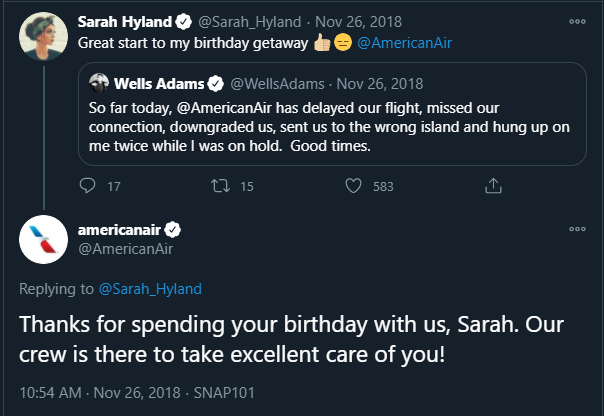
\includegraphics[width=9cm]{image6.png}}
\caption{AmericanAir Inappropriately Responds to Tweet Due to Misunderstood Sarcasm.}
\label{fig4}
\end{figure}


\begin{figure}[htbp]
\centerline{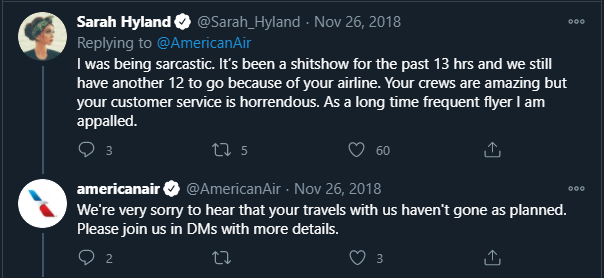
\includegraphics[width=9cm]{image7.png}}
\caption{AmericanAir Publicly Apologizes After Events in Fig 3 \& 4}
\label{fig5}
\end{figure}

Today, many state-of-the-art Sentiment Analysis services continue to serve results that do not detect sarcasm. This can be easily seen using Google Cloud’s Natural Language demo. In Figure 5 below, Google’s Sentiment system produces a score that is very positive for the statement “I love being ignored!”. Any human reader would immediately detect that this statement carries a strong negative sentiment, because no one likes to be ignored. \\

\begin{figure}[htbp]
\centerline{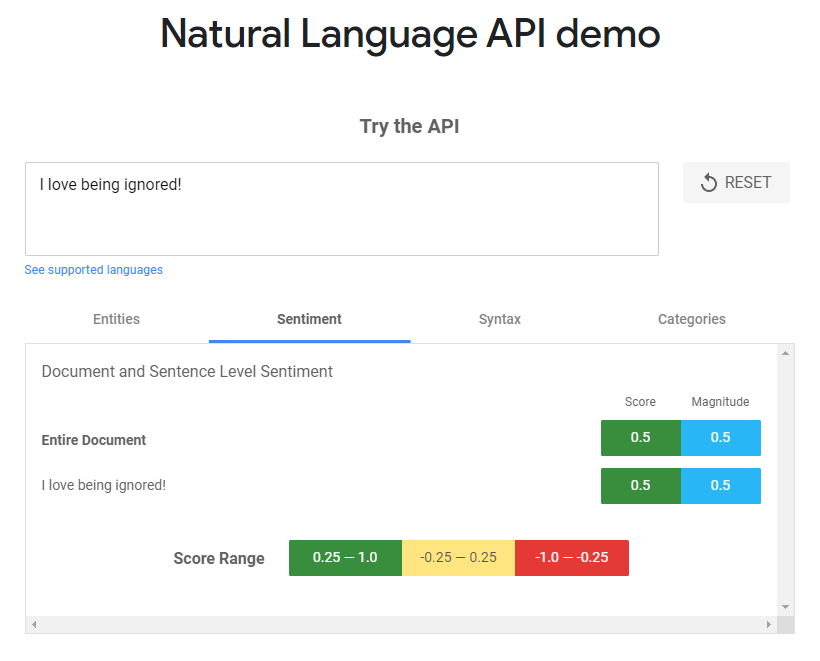
\includegraphics[width=9cm]{image8.png}}
\caption{Google Cloud’s Natural Language Demo}
\label{fig6}
\end{figure}

In the next section on related project works we will discuss what research efforts have been undertaken to address the current gap.\\

\section{Related Project Works}
There are many research papers on the topic of detecting sarcasm in Natural Language Processing (NLP) \cite{b3} \cite{b4}. Much of our inspiration came from Kaggle, a machine learning and data science social networking community. In particular, one Kaggle page \cite{b1} hosted the training data we used and linked to various other Kaggle member’s projects we looked at to come up with our approaches. One method in particular that caught our attention is word-embedding. This is a cutting edge NLP approach that allows algorithms to find similar words based on vector math. \\

Another site we found after we had started on our project is The Sarcasm Detector \cite{b2}. This web site hosts an application that is similar to our own. In reading the author's approach, they attempted three main techniques, sentiment deviation, n-grams, and general statics on most sarcastic topics. While we had already built our sentiment deviation algorithm before discovering this site, we decided to build our own n-gram algorithm after reading that this approach was the most successful for the author.\\
Our sentiment deviation algorithm has better success than our n-grams algorithm, which is the opposite of the author. There are additional approaches in papers such as looking at punctuation, capital letters, emojis, and just in general throwing machine learning at the problem without focusing on any particular feature. Many different approaches could have been tried, but the ones stated above are the approaches that seemed the most promising to our group. With additional time we could try more algorithms to see how they stack up against ours.\\

\section{Solution \& Analysis}
Our solution is an API endpoint where the user submits a piece of text and gets back a sentiment analysis score. Our endpoint internally makes calls to our sarcasm detection algorithms, which enable it to produce better results than current state-of-the-art sentiment analysis services in many cases. \\

\begin{figure}[htbp]
\centerline{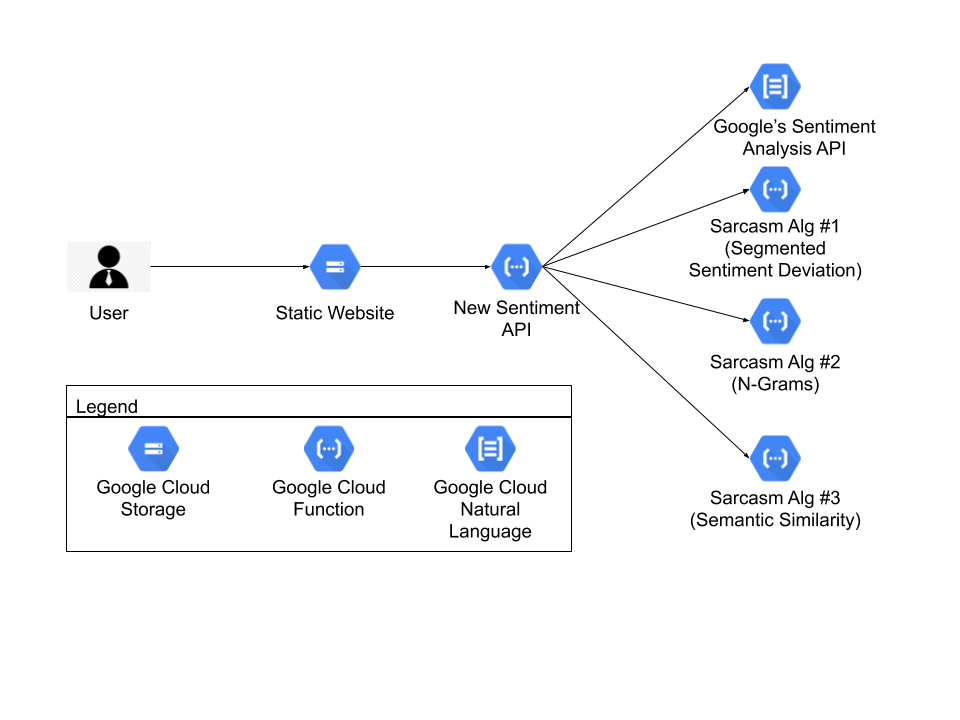
\includegraphics[width=9cm]{CS6221 Project Architecture Diagram-2.png}}
\caption{Project Architecture}
\label{fig6}
\end{figure}

Additionally, we built a web page for demonstration purposes that allows a user to enter text, submit it to the API, and see whether or not each sarcasm detection algorithm detected sarcasm, as well as the before and after sentiment scores. The “before” sentiment score is Google Cloud’s Natural Language Service Sentiment Analysis score. The “after” sentiment score is what our algorithm produced so users can see the difference that sarcasm detection makes in sentiment analysis.\\


\begin{figure}[htbp]
\centerline{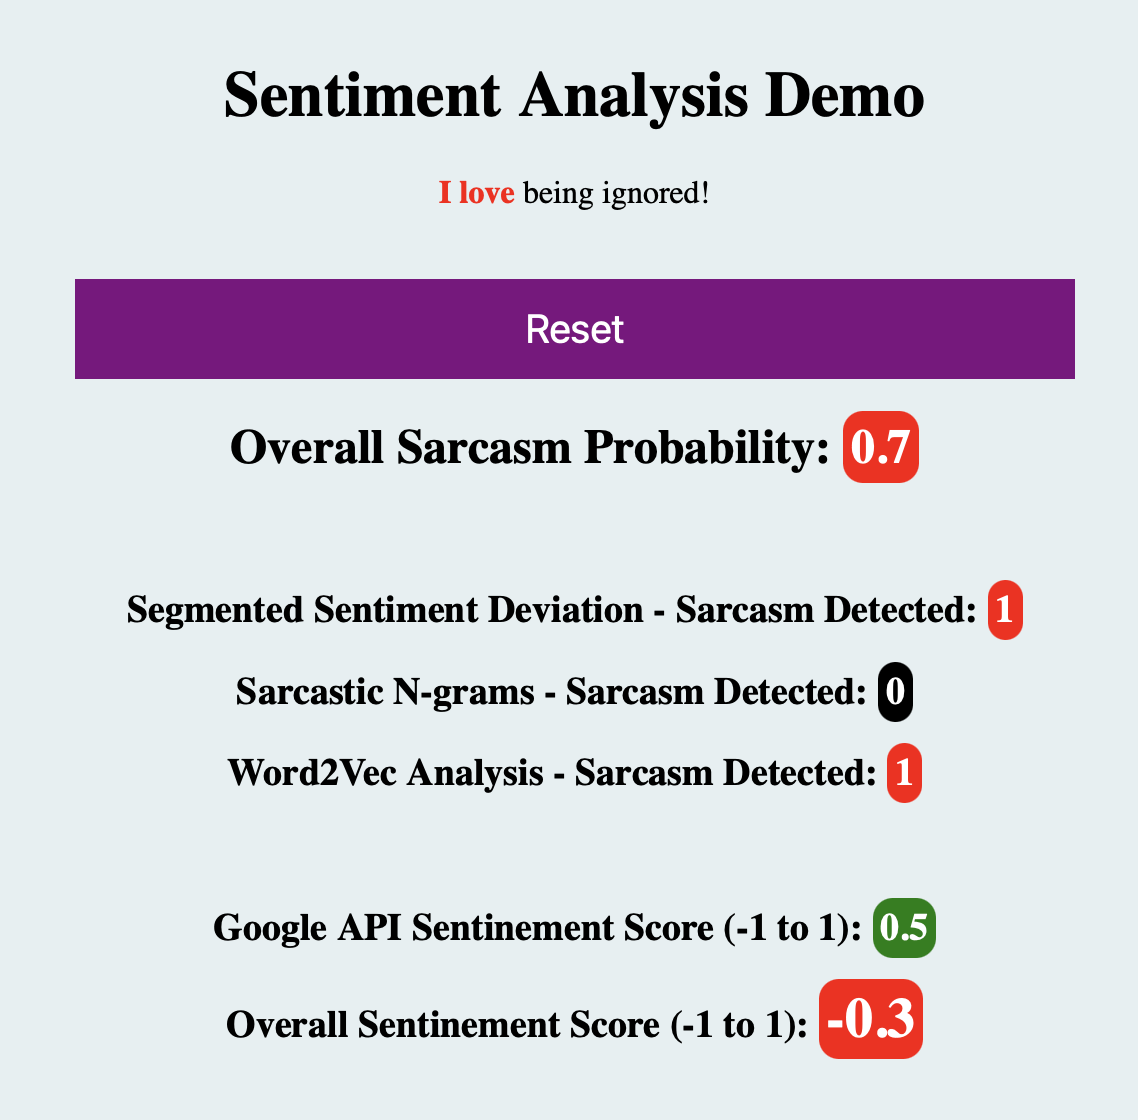
\includegraphics[width=7cm]{Screen Shot 2020-11-30 at 5.04.44 PM.png}}
\caption{Web Page For Live Demo}
\label{fig7}
\end{figure}





\subsection{Segmented Sentiment Deviation}
The Segmented Sentiment Deviation algorithm is based on the premise that sarcastic sentences are strongly emotional sentences where the sentiment of individual words fluctuate drastically and quickly in comparison to non-sarcastic sentences. The implementation of this algorithm utilizes Google’s Sentiment Analysis services by taking the input text, splitting it into individual words, and then feeding each word to Google’s service. This not only does the word based sentiment analysis for us, but it also returns a normalized sentiment score. After receiving the sentiment score of each word, the algorithm looks for strongly negative sentiment words and looks for strongly positive neighbors. We choose to consider neighbors up to five words away based on some preliminary analysis of our sarcasm dataset. If the algorithm finds a positive neighbor near the negative word, it flags the sentence as possibly being sarcastic. To reduce errors, we have defined strongly negative to mean a score of -0.5, and strongly positive to mean a score of 0.75, on a scale of -1 to 1. Thus the positive word has to be over the top, something like love, happy, excited, or overjoyed. \\

\begin{figure}[htbp]
\centerline{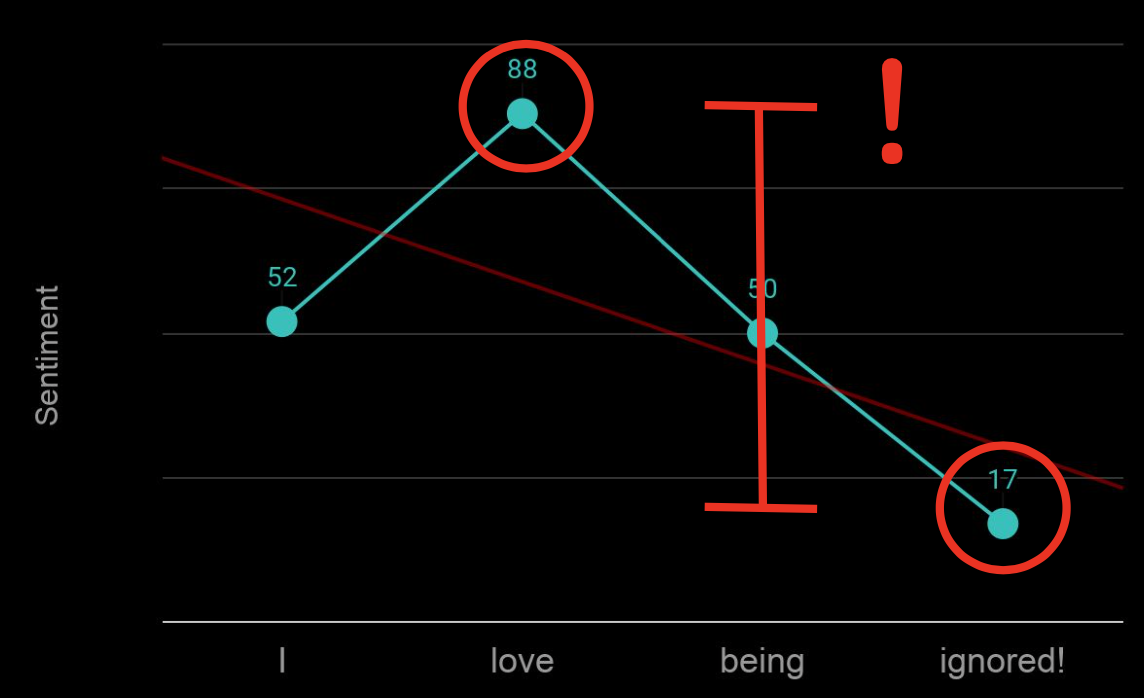
\includegraphics[width=7cm]{Screen Shot 2020-11-30 at 5.02.56 PM.png}}
\caption{Visualization Of Segmented Sentiment Deviation Algorithm}
\label{fig7}
\end{figure}

An example sentence that would trigger this algorithm is, “I love being ignored!” This is a great example because love is one of the most strongly positive words, and ignored is very negative. This very quick fluctuation in sentiment is a common tool that an author can employ to tell the reader that they feel exactly the opposite of what they have said. In fact the non-sarcastic version of this statement would likely use “hate” instead of “love.”  The sentiment deviation algorithm was tested on the same dataset as all the other algorithms. Each algorithm used a corpus of both sarcastic and non-sarcastic comment mined from Reddit \cite{b5}. This algorithm was 87.8\% accurate on non-sarcastic text, 16.8\% on sarcastic text, and overall was 52.3\% accurate on the combined corpus. This is somewhat low, but any score above 50\% overall is an improvement over what exists today. In all our algorithms we favored a conservative approach, giving up sarcasm accuracy to ensure that non-sarcasm accuracy didn’t fall below acceptable levels. \\
The biggest con of this algorithm is that it is an expert system as opposed to a machine learning system, and therefore it can not improve over time. Another issue we noticed is that Google’s sentiment scores on individual words doesn’t always seem to make sense. For example, using the following sarcastic comment from our dataset, “I guess there is *one* good thing for alcoholism gripping our youth.” the algorithm was unable to detect the presence of sarcasm. After further review it is because Google’s Sentiment Analysis service gave the word “alcoholism” a positive 0.3 score, instead of the strongly negative score we feel it deserves. “good” and “alcoholism” should have been contradictory scores triggering our algorithm, but it is out of scope in the project to start sentiment analysis from scratch. The biggest pro of this algorithm is that it can actually identify the words in the sentence that are sarcastic. In the previous example “love” was the sarcastic part of the sentence. In our demo we highlight the sarcastic word in red when this algorithm detects sarcasm. This is the only algorithm that we employed that is able to narrow sarcasm down to individual words. \\
\subsection{Sarcastic N-Grams}
The Sarcastic n-grams algorithm aims to statistically determine the most common set of words found in sarcastic remarks. An n-gram is simply a phrase made up of n words. Thus a bigram or 2-gram is two words, a trigram or 3-gram is three words, and the number can grow to any number n. In our algorithm we ended up choosing 4-grams and 5-grams. After trying many different n values, we discovered that higher n’s were less error prone. Higher n’s also led to a lower sarcasm detection rate, but a bigram or trigram had unacceptable accuracy scores on non-sarcastic sentences because the bi and tri grams were very generic. The most common n-grams were mined from the Reddit corpus \cite{b5}. Here are some sample 4-grams and 5-grams that were found to be most common for sarcastic sentences: “Am I the only”, “I would like to”, “I just want to”, “I would love to”, “This is what happens when”, “but at the same time”, “many many many many many.” \\

\begin{figure}[htbp]
\centerline{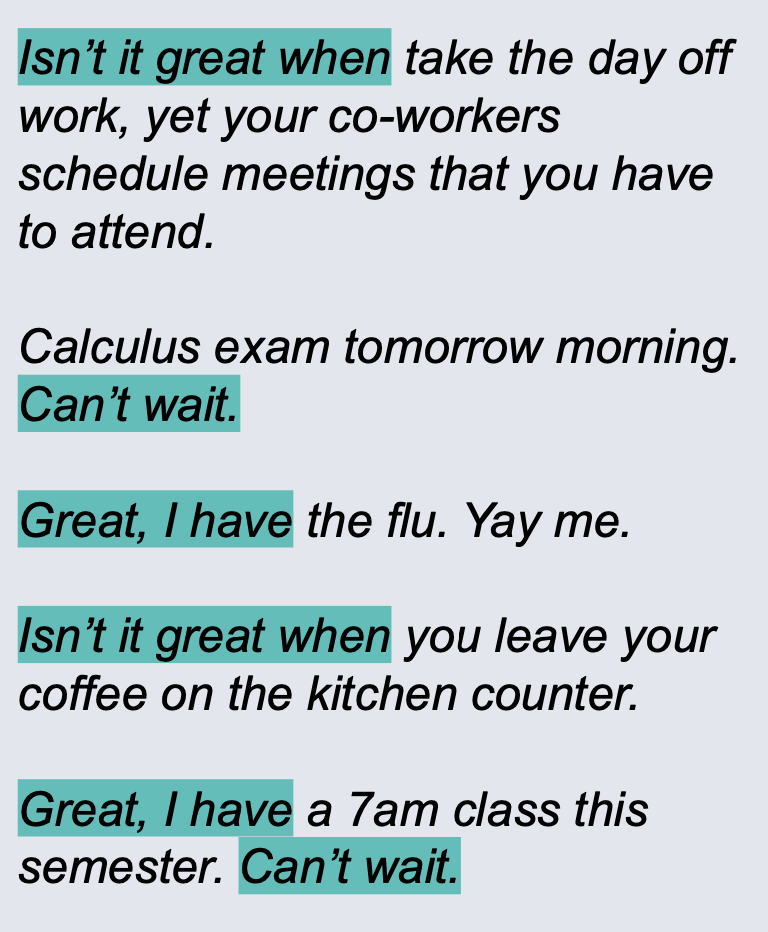
\includegraphics[width=7cm]{Screen Shot 2020-11-30 at 5.03.05 PM.png}}
\caption{Visualization Of Sarcastic N-Grams Algorithm}
\label{fig7}
\end{figure}

To reduce the number of false positives, the algorithm subtracts any n-grams that are also most common in non-sarcastic text, so that the final list contains the most common sarcasm n-grams that are not also common in non-sarcastic text. With this final list, the algorithm checks incoming text against the list to see if the input text contains a sarcasm n-gram. At a high level this algorithm aims to find an English vocabulary for sarcasm and see if that vocabulary exists in a new piece of material. This algorithm was tested the same way as all the other algorithms, using the Reddit corpus. It is worth mentioning that it is bad practice to train and test on the same data, but we do not have an alternative data source at this time. A future improvement for this algorithm would be to run it against a more varied data source. The n-gram algorithm was 90.2\% accurate on non-sarcastic text, 9.9\% on sarcastic text, and overall was 50.04\% accurate on the combined corpus. The overall accuracy of this algorithm is poor considering 50\% is the break even value for it to even be worth using. However, we believe that this algorithm shows promise in finding a sarcasm vocabulary and really just needs better training data to be effective. One main benefit of this algorithm is that it will improve with improved training data.\\
\subsection{Semantic Similarity}
The Semantic Similarity algorithm is based on the premise that sarcastic content will be more similar in meaning and semantic content to other sarcastic content than to non-sarcastic content.  The implementation of this algorithm involved using Word2Vec generated embeddings to determine the cosine similarities between an input text string and both a sarcastic and non-sarcastic corpus.  Word2Vec is a collection of ML algorithms published by Google \cite{b6}. Word2Vec uses neural networks to learn word associations and generate word embeddings.  These embeddings can then be used to calculate the ‘distance’ between two text strings or documents using several techniques, each of which provides a measure of similarity between the text.  \\

\begin{figure}[htbp]
\centerline{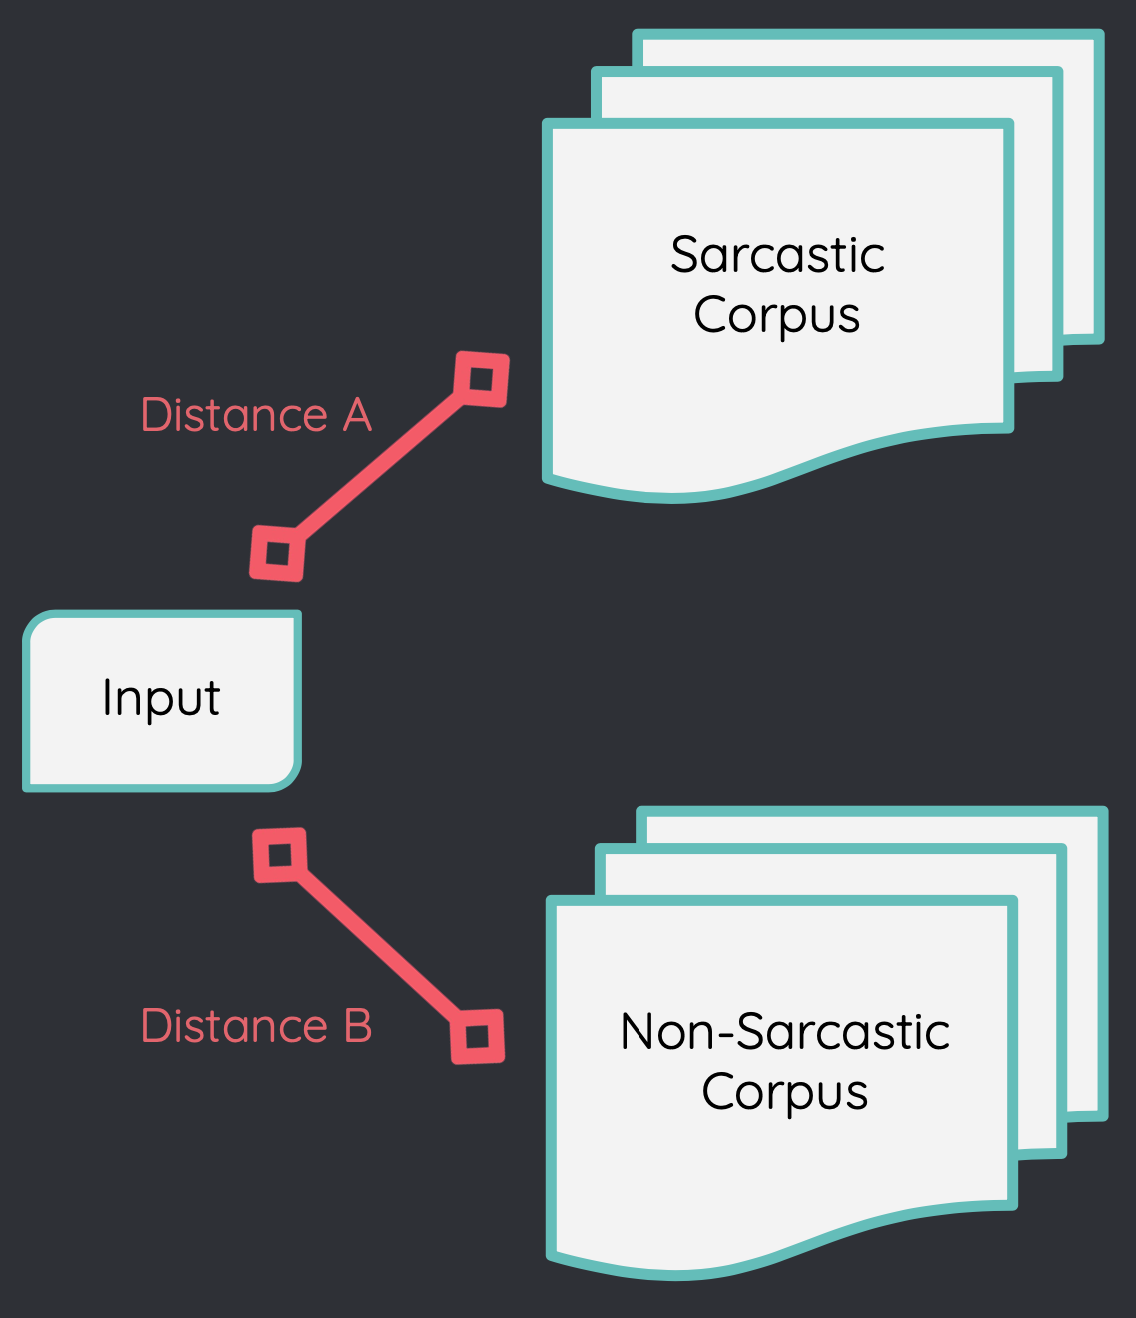
\includegraphics[width=7cm]{Screen Shot 2020-11-30 at 5.03.21 PM.png}}
\caption{Visualization Of Semantic Similarity Algorithm}
\label{fig7}
\end{figure}

We experimented with two techniques for calculating distance: Word Mover’s Distance and Cosine Similarity.  Once the Word2Vec vector space has been generated, Cosine Similarity is a straightforward Euclidean distance calculation.  Word Mover’s Distance, as outlined in this paper \cite{b7}, calculates the minimum Earth Mover’s Distance between each word in each of the texts.  Due to the resource intensity of a WMD calculation on large documents like ours, it would not be a viable API candidate (a single calculation takes several minutes), so we focused on Cosine Similarity.  \\ 
We used the Kaggle Reddit dataset to create a baseline sarcastic corpus of approximately 480,000 sarcastic comments and a baseline non-sarcastic corpus of approximately 480,000 comments.  The results in the table below were calculated using a test dataset comprising 20,000 sarcastic comments and 20,000 non-sarcastic comments.  Our algorithm calculated the Euclidean distance between each input and each of the two baseline corpora, and found that on average just over 60\% of the time the algorithm is able to correctly identify both sarcastic and non-sarcastic comments.\\

\begin{table}[htbp]
\caption{Accuracy By Algorithm}
\begin{center}
 \begin{tabular}{| c || c | c | c | } 
 \hline
Algorithm & Non Sarcastic & Sarcastic & Overall  \\ 
 \hline\hline
Segmented Sentiment& 87.8\% & 16.8\%  & 52.3\%   \\ 
 \hline
N-Grams& 90.2\%  & 9.9\%  & 50.04\%    \\[1ex] 
 \hline
Semantic Similarity& 60.1\%  & 62.3\%  & 61.2\%      \\[1ex] 
 \hline
\end{tabular}
\end{center}
\end{table}



These findings validate the initial premise that sarcastic content does in general bear more semantic similarity to non-sarcastic content, and vice versa.  While the overall accuracy is significantly higher than the other two approaches, the non-sarcastic accuracy is substantially lower, so this technique should not be used by itself to detect sarcasm. \\
One final key finding of note is that in cases where the algorithm correctly identified the input text, the average difference between the sarcastic and non-sarcastic corpora is 25\% larger than when the algorithm incorrectly identified the input.  This difference indicates it may be possible to weed out inputs that are likely to be incorrect, thus improving the accuracy of the output and relegating the filtered outputs to other methods if our sarcasm detection were implemented in a more elaborate ensemble manner.  We experimented with multiple versions of filtering out values where the difference in the distances is smallest and initial results indicate there is not a direct correlation between the difference in the distance between the corpora and the likelihood of an accurate identification.\\
\newline
\emph{Note on results in Table 1: These results are based on the methodology outlined in this paper, which is slightly different than what was shown in the live demo.  In the live demo, cosine similarity is calculated between the input text and a small sample of each of the two baseline corpora to prevent timeouts (runtime for a single calculation is 15 seconds on average).  Source code for both techniques is included with the project submission.  }

\section{Summary \& Future Work}
In conclusion, in the test environment using Reddit data where 50\% of the inputs are sarcastic, the Sentiment Analysis with Sarcasm Detection project outperformed Google’s API in percent of inputs correctly identified.  Further work should be done before the techniques outlined in this paper are applied to any real world situations because the percentage of sarcastic comments is likely to be much lower. (based on Reddit data only 1/10 of comments are sarcastic).  Future work could include: 
\begin{itemize}
\item \textbf{Creating Labeled Product Review Dataset.} Ideally we would’ve used a dataset with product reviews labeled as sarcastic.  Existing product review sets are unlabeled.
\item \textbf{N-Grams: Reapply Best Practices.}  Better training data should improve results, we could also more closely reapply the algorithm we drew inspiration from.
\item \textbf{Sentiment Similarity: Filter Candidate Inputs Likely To Fail.}  Certain distances seem more likely to be incorrect, further experimentation could prove this out.
\item \textbf{More Sophisticated Microservice Integration.}  Instead of weighting each algorithm equally, identify what types of inputs each is best at and then weight accordingly.


\begin{thebibliography}{00}
\bibitem{b1} https://www.kaggle.com/danofer/sarcasm
\bibitem{b2} http://www.thesarcasmdetector.com/
\bibitem{b3} https://web.stanford.edu/class/archive /cs/cs224n/cs224n.1194/reports/custom/15791781.pdf
\bibitem{b4} https://dl.acm.org/doi/abs/10.1145/1651461.1651471
\bibitem{b5} https://www.kaggle.com/danofer/sarcasm?select=train-balanced-sarcasm.csv
\bibitem{b6} https://code.google.com/archive/p/word2vec/
\bibitem{b7} http://proceedings.mlr.press/v37/kusnerb15.pdf
\end{thebibliography}
\vspace{12pt}

\end{document}
